\chapterimage{/3/head.jpg} % Chapter heading image
\chapter{Evoluzione termica dell'Universo}\label{3:ch}


\section{Temperatura e redshift}
La materia e la radiazione hanno avuto la stessa temperatura finché le interazioni sono state sufficientemente elevate per mantenere una condizione di equilibrio. Per verificare se questo accade si utilizza come tempo scala il tempo collisionale: $\tau_{coll}=(n c\sigma )^{-1}$. Oggi buona parte della materia è in forma neutra per cui possiamo assumere $\sigma \rightarrow \sigma_H$, inoltre  esprimere: $n_0 = \rho_0 / m_P$. Questa quantità va confrontata col tempo tipico di espansione dell'universo $\tau_{exp} \sim 1/H_0$. Si trova che, oggi, $\tau_{coll} \gg \tau_{exp}$, per cui $T_{m\, 0} \neq T_{r\, 0}$ e possiamo considerarle come componente separate.
L'andamento della temperatura in funzione del redshift si ricava tramite l'equazione di adiabaticità:
$$
\mathrm{d}(\rho c^2 a^3) = - p_m\: \mathrm{d}a^3
$$


\subsection{Temperatura della materia}
Si hanno due contributi alla densità di energia: l'energia di massa e l'energia termica. Per esprimere la pressione si fa uso dell'assunzione di gas perfetto. 
$$
 \rho c^2 = \rho_m c^2 + \frac{3}{2}k_B T_m \frac{\rho_m}{m_P} \qquad p_m = \frac{\rho_m k_B T_m}{m_P}
$$
Sostituendo questi valori nell'equazione di adiabaticità si ottiene:
\begin{equation}
    T_m = T_{m\, 0} (1+z)^2 = T_{m\, 0}\left ( \frac{a_0}{a}\right )^2  \propto a^{-2}
\end{equation}
Questo andamento era atteso poiché la condizione di adiabaticità implica $TV^{\gamma -1} = cost$, che per $\gamma=5/3$ restituisce lo stesso andamento appena ottenuto.

\subsection{Temperatura della radiazione}
In questo caso la densità di energia è ottenibile dalla funzione di corpo nero:
$$
 \rho_r c^2 = \sigma T_r^4 \qquad p_r = \frac{1}{3}\rho_r c^2 = \frac{\sigma T_r^4}{3}
$$
Sostituendo questi valori nell'equazione di adiabaticità si ottiene:
\begin{equation}
    T_r = T_{r\, 0} (1+z) = T_{r\, 0}\left ( \frac{a_0}{a}\right )  \propto a^{-1}
\end{equation}
Quindi materia e radiazione, quando separate, viaggiano su adiabatiche diverse.

Il tempo scala delle collisioni evolve come $\tau_{coll}=(nc\sigma)^{-1} \propto \rho_b^{-1}$. Dato che la densità dei barioni $\rho_b \propto (1+z)^{3}$ si ha che $\tau_{coll}\propto (1+z)^{-3}$. I tempi-scala in gioco (dalla \ref{eq:modelloeds}) sono quindi:
\begin{align*}
    & \tau_{coll} \propto (1+z)^{-3} \\
    & \tau_{exp, \, m} \propto (1+z)^{-3/2} \\
    & \tau_{exp, \, r} \propto (1+z)^{-2}
\end{align*}

Avvicinandosi al Big Bang, $\tau_{coll}\ll \tau_{exp}$, quindi la condizione di equilibrio è verificata. Inoltre andando a temperature più alte cambia la sezione d'urto $\sigma_H \rightarrow \sigma_T$ e la sezione d'urto Thomson è estremamente efficiente a fare collisioni e la materia diventa relativistica. Materia e radiazione erano quindi termicamente accoppiate. Esiste un valore di $z$ per cui si disaccoppiano, \textit{decoupling}, e vale circa $z_{dec}\approx 1000$. Con la temperatura che diminuisce si ha anche la ricombinazione (neutralizzazione) dell'idrogeno e si forma la superficie di ultimo scatter.

\section{Temperatura pre-disaccoppiamento}
Ci si aspetterebbe che, essendo materia e radiazione accoppiate, la temperatura evolva con un andamento intermedio tra le due, cioè $T\propto a^x$ con $x\in (-2, -1)$. L'accoppiamento è atteso osservando gli andamenti di $T_m$ e $T_r$ e assumendo che per $t<t_{decoup}$ la condizione $T_m = T_r$ venga mantenuta. 

Dalla condizione di adiabaticità, considerando tutti i contributi di materia e radiazione si ha:
\begin{equation}
    \mathrm{d} \left [ a^3    \left( \rho_m c^2 + \frac{3}{2}k_B T \frac{\rho_m}{m_P} + \sigma T^4 \right)  \right] = - \mathrm{d} \left [ a^3    \left( \frac{\rho_m k_B T_m}{m_P} + \frac{\sigma T_r^4}{3}  \right)  \right]
\end{equation}

Introducendo la quantità adimensionale:
\begin{equation}
    \sigma_{r}= \frac{4}{3} \frac{m_P ~\sigma ~T^3}{k_B ~\rho_m}
\end{equation}

e ricordando che $\mathrm{d} (\rho_m a^3) = 0$, si può ottenere la relazione:
\begin{equation}
\frac{ \mathrm{d}T}{T}= - \frac{ \mathrm{d}a}{a} \: \frac{1+\sigma_{r}}{\frac{1}{2} +\sigma_{r}}
\end{equation}

Dal momento che la quantità $\sigma_{r}$ dipende dal tempo e dalla temperatura, non è sempre possibile risolvere analiticamente questa equazione. Si può però verificare che, dopo il disaccoppiamento ($T\to T_{r}$), il valore $\sigma_{r}=cost=\sigma_{r \, 0}$. In particolare si ottiene:
\begin{equation*}
    \sigma_{r \, 0} \simeq 1.35 \cdot 10^8 \; (\sigma_{b\, 0}h^2)^{-1}
\end{equation*}

Il fatto che $\sigma_{r}$ sia costante ed estremamente alto, garantisce che l'andamento al momento del disaccoppiamento sia $\mathrm{d}T / T \propto \mathrm{d}a / a$ per cui per $t<t_{decoup}$ si ha: 
\begin{equation}
T \propto (1+z) \propto a^{-1} 
\end{equation}

A maggior ragione per $t$ piccoli, a causa dell'aumento di $T$, emerge sempre di più il comportamento relativistico della materia. Quindi, a differenza di quanto era atteso, è solo il comportamento della radiazione a dominare a queste epoche (Fig. \ref{fig:3logzt}).
\begin{figure}[ht]
    \centering
    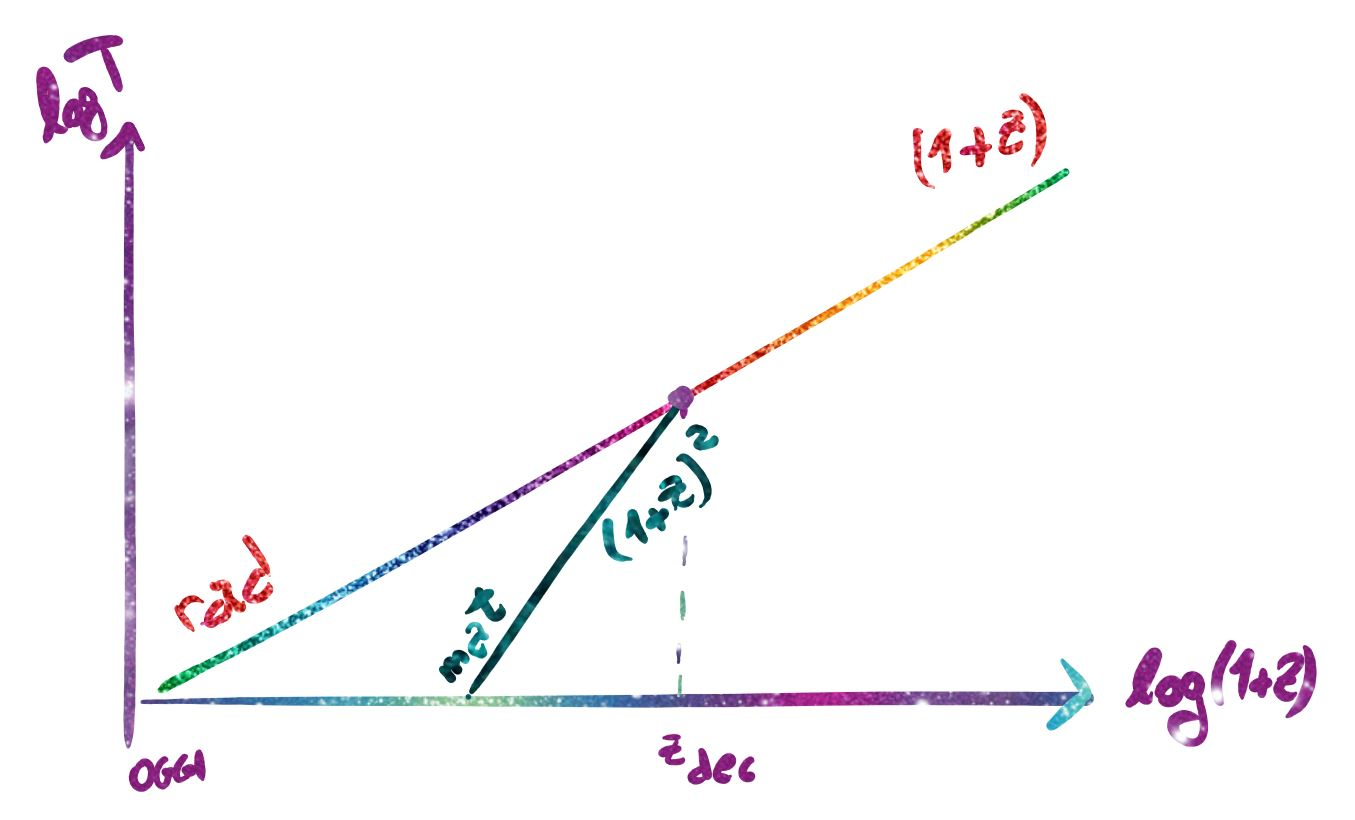
\includegraphics[width=.85\textwidth]{Pictures/3/logT-z.jpg}
    \caption{Andamento della temperatura di materia e radiazione pre e post disaccoppiamento.}
    \label{fig:3logzt}
\end{figure}

La quantità $\sigma_{r}$ viene detta \textit{entropia della radiazione per barione}, corrisponde infatti al rapporto fra la densità di entropia della radiazione $S_r= (\rho c^2 + p_r)/T$ e il numero dei barioni esistenti (reso adimensionale dividendo per $k_B$). Quindi si ha che ``c'è un sacco di entropia nella radiazione rispetto al numero di particelle barioniche nell'universo''. Questo concetto può anche essere visto studiando la densità di capacità termica $\mathfrak{C}$:
$$
\rho_r ~\mathfrak{C}:=\frac{\partial \left (\rho_r ~c^2  \right )}{\partial T}=4\sigma T^3 \qquad\qquad \rho_m ~\mathfrak{C}:=\frac{\partial\left ( \frac{3}{2}\frac{\rho_m k_B T}{m_P}  \right )}{\partial T} = \frac{3}{2}\frac{\rho_m k_B}{m_p}
$$
Il rapporto tra queste due quantità corrisponde proprio a $2\sigma_{r}$. Questo ci sta dicendo che la capacità termica è dominata dalla componente radiativa.
Inoltre si introduce un parametro importante, $\eta$:
\begin{equation}
    \eta := \frac{\# ~nucleoni}{\# ~fotoni} = \frac{\rho_b}{m_p} \frac{1}{ \left( \frac{k_B T}{\hslash c}\right)^3 \int \frac{8 \pi \lambda^2}{e^x - 1} \mathrm{d}x} \propto \frac{\rho_m}{m_P T^3}
\end{equation}

In particolare si ha:
\begin{equation}
    \sigma_{r \, 0 } = 3.6 ~ \eta_0^{-1}
\end{equation}

Il valore grande di $\sigma_{r}$ è dovuto al fatto che oggi il numero di fotoni è circa $10^8$ volte il numero di nucleoni (motivo per cui la capacità termica della radiazione è maggiore). Questo è strettamente legato ad un fenomeno accaduto nell'universo primordiale: l'\textbf{anisotropia barioni-antibarioni}. Sotto l'ipotesi di conservazione del numero barionico vale la relazione $(n_b - n_{\overbar{b}} )~a^3 = n_{b \,0}~a_0^3$ poiché oggi non osserviamo antibarioni. Come verrà discusso, nell'univeso primordiale $n_b \simeq n_{\overbar{b}} \simeq n_\gamma $, dove $n_\gamma $ è il numero dei fotoni; una quantità adimensionale per misurare l'anisotropia è:
\begin{equation}
    \frac{n_b - n_{\overbar{b}}}{n_b + n_{\overbar{b}}}= \frac{n_b - n_{\overbar{b}}}{2 n_\gamma} \equiv \frac{n_{b \,0}}{2n_{\gamma \,0}} \propto \sigma_{r \, 0 }^{-1}
\end{equation}
Questo implica che nell'universo primordiale il numero di barioni e antibarioni non era esattamente uguale: a causa della piccola differenza sono sopravvissuti i pochi barioni in un mare di fotoni prodotti per annichilazione. Per esempio: $10^8$ fotoni $+$ $10^8$ antibarioni $+$ $(10^8 +1)$ barioni avrebbero generato $3\cdot 10^8$ fotoni e $1$ barione, valore simile al rapporto osservato. Quali sono i meccanismi in grado di produrre una sì piccola differenza tra $b$ e $\overbar{b}$?

\newpage
La temperatura verrà utilizzata come cronometro per studiare la storia evolutiva dell'universo, infatti è in base a essa che si sceglie quale fisica utilizzare. Per qualsiasi particella di massa $m$ esiste sempre una $T_{eq}$ alla quale l'energia termica $k_BT_{eq}$ è uguale all'energia di massa $2m c^2$. Una coppia elettrone-positrone può esistere soltanto se $T\gtrsim T_{eq}$ altrimenti dominerebbe il processo di annichilazione (produzione di 2 fotoni). Dalla relazione si può concludere che \textbf{a temperature elevate (universo primordiale) possono soltanto esistere particelle di grande massa}. Dal Big Bang ad oggi sarà possibile, semplificando, distinguere l'era adronica e poi l'era leptonica.

\vspace{1em}
I due momenti fondamentali fino ad ora discussi sono:
\begin{example}[Equivalenza Materia-Radiazione]
    $\rho_m (z_{eq})=\rho_r(z_{eq})$
\end{example}
Precedentemente si è ricavato: $1+z_{eq}=\Omega_{0m}/\Omega_{r\, 0}$, dove per $\Omega_{r\, 0}$ si include anche la componente relativistica della materia (e.g. neutrini). Dalla relazione tempo-redshift:
$$
t_{eq} \approx 10^4 ~\mathrm{yr} \qquad\qquad z \approx 5000
$$
L'epoca dominata dalla radiazione è un'inezia! Le equazioni di Friedmann per la sola materia non portano a grossi errori di calcolo.

\begin{example}[Disaccoppiamento]
    Tempo dopo il quale $T_m(t)\neq T_r(t)$
\end{example}
Quando la temperatura scende sotto una certa soglia si forma idrogeno neutro e $\sigma_T \rightarrow \sigma_H$. Questo avviene a:
$$
t_{dec} \approx 3\cdot 10^5 ~\mathrm{yr} \qquad\qquad z \approx 1000
$$
Il realtà si vedrà che il tempo a cui avviene la ricombinazione è diverso dal tempo a cui avviene il disaccoppiamento e dipende dalle specie chimiche considerate.

